\documentclass[10pt]{beamer}
% \documentclass[handout,10pt]{beamer}
\usepackage{my_style}
%%%%%%%%%%%%%%%%%%%%%%%%%%%%%%%%%%%%%%%%%%%%%%%%%%%%%%%%%%%%%%%%%%%%%%%%


\title[Math/CS 375]{Lecture 12 - B}
\subtitle{ \S 5.4 Generalized Gaussian Quadrature}

\begin{document}
% -------------------------------------------------
\begin{frame}
  \titlepage
\end{frame}

%%%%%%%%%%%%%%%%%%%%%%%%%%%%%%%%%%%%%%%%%%%
\begin{frame}{Goals}
We will answer these questions:\\[3mm]
\begin{itemize}
    \item How do we apply Gauss quadrature on multiple subintervals?
    \item How do we construct rules with more than two nodes?
    \item Why do $m$ nodes give degree of precision $2m-1$?
    \item How do nodes and subintervals affect accuracy and cost?
\end{itemize}
\end{frame}



%%%%%%%%%%%%%%%%%%%%%%%%%%%%%%%%%%%%%%%%%%%%%%%%%%%%%%%%%%%%%%%%%%%%%%%%%
\sectionframe{Composite Gauss}
%%%%%%%%%%%%%%%%%%%%%%%%%%%%%%%%%%%%%%%%%%%%%%%%%%%%%%%%%%%%%%%%%%%%%%%%
\begin{frame}{Using Trapezoid Twice}

    \cols{
        \centering
    \begin{tikzpicture}[scale=0.5]
    \begin{axis}[
        width=10cm, height=6cm,
        xlabel={$x$}, ylabel={$y$},
        grid=major, 
        thick,
        domain=0:2,
        samples=100,
    ]
        % Define and plot the function f(x) = sin(x)
        \addplot[name path=func, color=blue, thick, domain=-1:1] {2*x*(x-0.5)*(x+0.25)+3};
    
        % Define the x-axis path from x=0 to x=1.5
        \addplot[name path=xaxis, draw=none, domain=-1:1] {0};
    
        % Shade the area under f(x) between x=0 and x=1.5
        \addplot [
            fill=blue!20,    % Fill color
            fill opacity=0.3, % Adjust opacity here
            draw=none
        ] fill between [
            of=func and xaxis,
            soft clip={domain=-1:1},
        ];
        
    \end{axis}
    \end{tikzpicture}\\
    Exact integral over $[-1,1]$
    
    }{
    \centering
  \begin{tikzpicture}[scale=0.5]
\begin{axis}[
    width=10cm, height=6cm,
    xlabel={$x$}, ylabel={$y$},
    grid=major, 
    thick,
    domain=0:2,
    samples=100,
]
    \addplot[name path=func, color=blue, thick, domain=-1:1] {2*x*(x-0.5)*(x+0.25)+3};

    \addplot[name path=xaxis, draw=none, domain=-1:1] {0};

    \addplot[name path=int, sharp plot, dashed, thick]
        coordinates {(-1, 0.75) (0, 3) (1,4.25)};

    \addplot[
        fill=blue!20,
        fill opacity=0.3,
        draw=none
    ] fill between [
        of=int and xaxis,
        soft clip={domain=-1:1},
    ];

    \addplot[mark=*, only marks, color=red]
        coordinates {(-1, 0.75) (0, 3) (1,4.25)};
\end{axis}
\end{tikzpicture}
    Composite Trapezoid 
    }
    \vspace{3mm}
    \begin{itemize}
        \item Each subinterval is called a \textbf{panel}.
        \item \textbf{Composite Trapezoid} uses one trapezoid per panel.
        \item We can apply the same idea to Gaussian quadrature
    \end{itemize}
\end{frame}

%%%%%%%%%%%%%%%%%%%%%%%%%%%%%%%%%%%%%%%%%%%%%%%%%%%%%%%%%%%%%%%%%%%%%%%%
\begin{frame}{Using Gauss Quadrature Twice}
    \begin{itemize}
        \item Apply Gauss quadrature on each panel separately
        \item Compare the composite Trapezoid vs. composite Gauss visually 
    \end{itemize}
        \vspace{5mm}
    \cols{
        \centering
        \begin{tikzpicture}[scale=0.5]
        \begin{axis}[
            width=10cm, height=6cm,
            xlabel={$x$}, ylabel={$y$},
            grid=major, 
            thick,
            domain=0:2,
            samples=100,
        ]
            % Define and plot the function f(x) = sin(x)
            \addplot[name path=func, color=blue, thick, domain=-1:1] {2*x*(x-0.5)*(x+0.25)+3};
    
            % Define the x-axis path from x=0 to x=1.5
            \addplot[name path=xaxis, draw=none, domain=-1:1] {0};
        
            \addplot[name path=int, sharp plot, dashed, thick] coordinates {(-1, 0.75) (0, 3) (1,4.25)};

            \draw[dashed,thin] (axis cs:0,-1) -- (axis cs:0,6);

     
            \addplot [
                fill=blue!20,    % Fill color
                fill opacity=0.3, % Adjust opacity here
                draw=none
            ] fill between [
                of=int and xaxis,
                soft clip={domain=-1:1},
            ];
            % Mark points x=0 and x=1.5 on the curve
            \addplot[mark=*, only marks, color=red] coordinates {(-1, 0.75) (0, 3) (1,4.25)};
        \end{axis}
        \end{tikzpicture}
        Composite Trapezoid 
    
    }{
        \centering
        \begin{tikzpicture}[scale=0.5]
        \begin{axis}[
            width=10cm, height=6cm,
            xlabel={$x$}, ylabel={$y$},
            grid=major, 
            thick,
            domain=-1:1,
            samples=100,
        ]
            % Define and plot the function f(x)
            \addplot[name path=func, color=blue, thick, domain=-1:1] {2*x*(x - 0.5)*(x + 0.25) + 3};

            % Define the x-axis path from x=-1 to x=1
            \addplot[name path=xaxis, draw=none, domain=-1:1] {0};

            % Gauss-Legendre points for n=2 over [-1,0] and [0,1]
            % For standard interval [-1,1], the Gauss points are at x = ±1/√3
            % Map these points to each subinterval

            % First subinterval [-1,0]
            \pgfmathsetmacro{\a}{-1}
            \pgfmathsetmacro{\b}{0}
            \pgfmathsetmacro{\xiA}{\a + (\b - \a)*(1 - 1/ sqrt(3))/2}
            \pgfmathsetmacro{\xiB}{\a + (\b - \a)*(1 + 1/ sqrt(3))/2}
            \pgfmathsetmacro{\fxiA}{2*\xiA*(\xiA - 0.5)*(\xiA + 0.25) + 3}
            \pgfmathsetmacro{\fxiB}{2*\xiB*(\xiB - 0.5)*(\xiB + 0.25) + 3}

            % Second subinterval [0,1]
            \pgfmathsetmacro{\c}{0}
            \pgfmathsetmacro{\d}{1}
            \pgfmathsetmacro{\xiC}{\c + (\d - \c)*(1 - 1/ sqrt(3))/2}
            \pgfmathsetmacro{\xiD}{\c + (\d - \c)*(1 + 1/ sqrt(3))/2}
            \pgfmathsetmacro{\fxiC}{2*\xiC*(\xiC - 0.5)*(\xiC + 0.25) + 3}
            \pgfmathsetmacro{\fxiD}{2*\xiD*(\xiD - 0.5)*(\xiD + 0.25) + 3}

            % Plot vertical lines at the subinterval boundaries
            \draw[dashed,thin] (axis cs:0,-1) -- (axis cs:0,6);

            % Mark the Gauss points
            \addplot[mark=*, only marks, color=red] coordinates {
                (\xiA,\fxiA) 
                (\xiB,{2*(\xiB)*(\xiB - 0.5)*(\xiB + 0.25) + 3})
                (\xiC,{2*(\xiC)*(\xiC - 0.5)*(\xiC + 0.25) + 3})
                (\xiD,{2*(\xiD)*(\xiD - 0.5)*(\xiD + 0.25) + 3})
            };

            % Draw vertical dashed lines from x-axis to function at Gauss points
            \draw[dashed] (axis cs:\xiA,0) -- (axis cs:\xiA,{2*(\xiA)*(\xiA - 0.5)*(\xiA + 0.25) + 3});
            \draw[dashed] (axis cs:\xiB,0) -- (axis cs:\xiB,{2*(\xiB)*(\xiB - 0.5)*(\xiB + 0.25) + 3});
            \draw[dashed] (axis cs:\xiC,0) -- (axis cs:\xiC,{2*(\xiC)*(\xiC - 0.5)*(\xiC + 0.25) + 3});
            \draw[dashed] (axis cs:\xiD,0) -- (axis cs:\xiD,{2*(\xiD)*(\xiD - 0.5)*(\xiD + 0.25) + 3});

            \addplot[name path=p0, color=black, thick,dashed, domain=-1:0] { (\fxiB - \fxiA)/(\xiB-\xiA)*(x - \xiA) + \fxiA};
            \addplot[name path=p1, color=black, thick,dashed, domain=0:1] { (\fxiD - \fxiC)/(\xiD-\xiC)*(x - \xiC) + \fxiC};

            \addplot [
                fill=blue!20,    % Fill color
                fill opacity=0.3, % Adjust opacity here
                draw=none
            ] fill between [
                of=p0 and xaxis,
                soft clip={domain=-1:0},
            ];
            \addplot [
                fill=blue!20,    % Fill color
                fill opacity=0.3, % Adjust opacity here
                draw=none
            ] fill between [
                of=p1 and xaxis,
                soft clip={domain=0:1},
            ];
        
        \end{axis}
        \end{tikzpicture}
        Composite Gauss 
    }
    \vspace{3mm}

\end{frame}
%%%%%%%%%%%%%%%%%%%%%%%%%%%%%%%%%%%%%%%%%%%%%%%%%%%%%%%%%%%%%%%%%%%%%%%%%
\begin{frame}{Composite Gauss}

\begin{itemize}
    \item Composite Trapezoid has a neat formula 
    $$
    \int_a^b f(x)\,dx \approx    h    \left(\frac{1}{2} f(x_0) +   f(x_1) +  f(x_2) + \dots +   f(x_{N-1}) + \frac{1}{2} f(x_N)\right)
    $$
        \vfill 
    \item Composite Gauss adds the contributions from interior nodes on each panel.
        \vfill 
    \question{How do you implement composite Gauss?}
\end{itemize}
    
\end{frame}
%%%%%%%%%%%%%%%%%%%%%%%%%%%%%%%%%%%%%%%%%%%%%%%%%%%%%%%%%%%%%%%%%%%%%%%%%
\begin{frame}{Implementation}
\begin{enumerate}
    \item Divide $[a,b]$ into $N$ equal panels:
    \[
        h=\frac{b-a}{N}, \qquad x_i=a+ih,\quad i=0,\ldots,N.
    \]
    \item Map the standard Gauss nodes to panel $[x_i,x_{i+1}]$:
    \[
        x(t)=\frac{x_i+x_{i+1}}{2}+\frac{h}{2}t.
    \]
    \item Apply two-point Gauss on each panel:
    \[
        I_i=\frac{h}{2}\left[
        f\left(x\left(-\frac{1}{\sqrt{3}}\right)\right)
        +f\left(x\left(\frac{1}{\sqrt{3}}\right)\right)\right].
    \]
    \item Add the results: $\displaystyle I\approx\sum_{i=0}^{N-1} I_i$.
\end{enumerate}
\end{frame}


\begin{frame}[fragile]{Modular Implementation}

\begin{itemize}
    
    \item Implement gauss over any interval $[a,b]$
\begin{lstlisting}[mathescape]
I = gauss(f,a,b)
\end{lstlisting}

    \item Choose a partition 
    $$
        P=\{x_0,x_1,\dots,x_N\}
    $$

    \item Call your code in a loop
\begin{lstlisting}[mathescape]
S = 0
for $i=0$ to $N-1$
  S = S + gauss(f,$x_i$,$x_{i+1}$)
end
\end{lstlisting}
\end{itemize}
\end{frame}


%%%%%%%%%%%%%%%%%%%%%%%%%%%%%%%%%%%%%%%%%%%%%%%%%%%%%%%%%%%%%%%%%%%%%%%%%
\begin{frame}{Composite Gauss}
    \method{Composite Gauss}
    {function $f(x)$, interval $[a,b]$, number of panels $N$}
    {Approximate integral $\int_a^b f(x)\,dx$}
    {Create $N$ equal panels and add up two-point Gauss quadratures for each panel}
    \vspace{3mm}
    \begin{itemize}
        \item Adjacent Gauss panels do not share endpoint evaluations.
        \item Composite Gauss is implemented \textit{modularly}
    \end{itemize}
\end{frame}


%%%%%%%%%%%%%%%%%%%%%%%%%%%%%%%%%%%%%%%%%%%%%%%%%%%%%%%%%%%%%%%%%%%%%%%%%
\sectionframe{Gauss Quadrature Theorem}
%%%%%%%%%%%%%%%%%%%%%%%%%%%%%%%%%%%%%%%%%%%%%%%%%%%%%%%%%%%%%%%%%%%%%%%%%
\begin{frame}{Goal}

\begin{itemize}
    \item We have derived \textit{two-point} Gauss 
    \begin{eqnarray*}
  \int_{-1}^1 f(x) \; \mathit{dx} \approx f\left(-\frac{\sqrt{3}}{3}
  \right) + f\left(\frac{\sqrt{3}}{3} \right)
\end{eqnarray*}

    \item Next, we learn the general $m$-point Gauss rule.
    In the theorem, we write $m=n+1$:
$$\int_a^b f(x)\,dx  \approx  \sum_{i=0}^n w_i f(x_i) $$

\end{itemize}
    \vfill 
\begin{block}{Goal}
    Learn the \textbf{Gaussian Quadrature Theorem}.
\end{block}
\end{frame}
%%%%%%%%%%%%%%%%%%%%%%%%%%%%%%%%%%%%%%%%%%%%%%%%%%%%%%%%%%%%%%%%%%%%%%%
\begin{frame}{Three-Point Gauss Quadrature}
\[
\int_{-1}^{1} f(x)\,dx \approx
\frac{5}{9}f\left(-\sqrt{\frac{3}{5}}\right)
+\frac{8}{9}f(0)
+\frac{5}{9}f\left(\sqrt{\frac{3}{5}}\right).
\]
\begin{itemize}
    \item Three nodes give degree of precision $5$.
    \item Simpson's rule also uses three nodes, but has degree of precision $3$.
\end{itemize}
\begin{block}{General Result}
An $m$-point Gauss rule is exact for every polynomial of degree at most $2m-1$.
\end{block}
\question{Where do these nodes and weights come from?}
\end{frame}

\begin{frame}{Inner Product}

\begin{itemize}
    \item We know the \textbf{inner product} of vectors  $u$ and $v$ 
        $$ u^Tv  = \sum_{i=1}^n u_iv_i$$
    \item Functions $f(x)$ and $g(x)$ are like  ``infinite dimensional vectors"

    \define{Inner Product}{
        Let $f(x)$, $g(x) \in C([a,b])$. The \textbf{inner product} of the functions is 
        $$
        \int_a^b f(x)\,g(x)\,dx
        $$
    
    }
    
        
\end{itemize}
\end{frame}
%%%%%%%%%%%%%%%%%%%%%%%%%%%%%%%%%%%%%%%%%%%%%%%%%%%%%%%%%%%%%%%%%%%%%%%

\begin{frame}{Orthogonal Functions}


\define{Orthogonal functions}{
Two functions $f(x)$ and $g(x)$ are \textbf{\emph{orthogonal}} on $[a,b]$ if
\begin{equation*}
\int_{a}^{b} f(x)g(x)\,dx = 0
\end{equation*}
}
\begin{itemize}
    \item Example: $f(x) = x$, $g(x) = x^2-1$ on the interval $[-1,1]$

    \item Inner product
    \begin{align*}        
        \int_{-1}^1 f(x)g(x)\,dx &= \int_{-1}^1 x(x^2-1)\,dx \\
         &= \int_{-1}^1 (x^3-x)\,dx \\
         &=  \left.\frac{1}{4}x^4-\frac{1}{2}x^2\right|_{-1}^1=0 \\
    \end{align*}

\end{itemize}
    
\end{frame}

% Main lecture proof: three key steps. Detailed reference slides follow.
\begin{frame}{Proof: Split the Polynomial}
\framesubtitle{Step 1: Reduce to a low-degree remainder}
\begin{itemize}
    \item Let $f$ have degree at most $2m-1$.
    \item Choose a degree-$m$ polynomial $q$ orthogonal to every
    polynomial of degree at most $m-1$.
    \item Use the $m$ roots of $q$ as the quadrature nodes.
\end{itemize}
\begin{block}{Polynomial Division}
\[
    f(x)=p(x)q(x)+r(x),
    \qquad \deg p\le m-1,\quad \deg r\le m-1.
\]
Here $p$ is the quotient and $r$ is the remainder.
\end{block}
\keyidea{The remainder $r$ is low enough degree to interpolate exactly
using $m$ nodes.}
\end{frame}

\begin{frame}{Proof: Both Ignore the Same Part}
\framesubtitle{Step 2: The product $pq$ contributes zero}
Recall $f=pq+r$.
\begin{columns}[T]
\begin{column}{0.48\textwidth}
\begin{block}{The Integral}
Orthogonality gives
\[
    \int_a^b p(x)q(x)\,dx=0.
\]
Therefore,
\[
    \int_a^b f(x)\,dx=\int_a^b r(x)\,dx.
\]
\end{block}
\end{column}
\begin{column}{0.48\textwidth}
\begin{block}{The Quadrature}
The nodes are roots of $q$:
\[
    q(x_i)=0.
\]
Therefore,
\[
    f(x_i)=r(x_i).
\]
\end{block}
\end{column}
\end{columns}
\vspace{3mm}
\keyidea{Both the integral and the quadrature depend only on $r$.}
\end{frame}

\begin{frame}{Proof: Integrate the Remainder Exactly}
\framesubtitle{Step 3: The remainder has degree at most $m-1$}
The interpolant through the $m$ nodes equals $r$:
\[
    r(x)=\sum_{i=1}^{m} r(x_i)\ell_i(x).
\]
Choose the weights by integrating the Lagrange basis:
\[
    w_i=\int_a^b\ell_i(x)\,dx
    \quad\Longrightarrow\quad
    \int_a^b r(x)\,dx=\sum_{i=1}^{m}w_i r(x_i).
\]
Thus,
\[
    \boxed{\int_a^b f(x)\,dx
    =\int_a^b r(x)\,dx
    =\sum_{i=1}^{m}w_i r(x_i)
    =\sum_{i=1}^{m}w_i f(x_i).}
\]
\keyidea{Both ignore $pq$ and integrate the remainder $r$ exactly.}
\end{frame}

% Reference material: may be skipped during the lecture.
\begin{frame}{Reference: Gauss Quadrature Theorem}
\framesubtitle{Notation in these reference slides: $m=n+1$, $w_i=A_i$}
Gauss proved the following result:

\begin{block}{Theorem}
Let $q(x)$ be a nontrivial polynomial of degree $n+1$ such that
\begin{equation*}
    \int_{a}^{b} x^k q(x) dx = 0 \qquad (0\le k \le n)
\end{equation*}
and let $x_0, x_1, \ldots, x_n$ be the zeros of $q(x)$.  Then the quadrature
\begin{equation*}
  \int_{a}^{b} f(x)dx \approx \sum_{i=0}^n A_i f(x_i), \text{ where } A_i=\int_{a}^{b} \ell_i(x) dx
\end{equation*}
is exact for all polynomials of degree at most $2n+1$. 
\end{block}

\vspace{1em}

Recall $\ell_i(x)$ is the $i$th \textbf{Lagrange basis function}.  Here, $\ell_i(x)$ is
   defined \\with respect to the $x_0, x_1, \ldots, x_n$ zeros of $q(x)$. 

\end{frame}
%%%%%%%%%%%%%%%%%%%%%%%%%%%%%%%%%%%%%%%%%%%%%%%%%%%%%%%%%%%%%%%%%%%%%%%%%
\begin{frame}[shrink]{Reference: Variables and Assumptions}

\begin{table}[h]
    \centering
    \begin{tabular}{|c|p{9cm}|}
        \hline
        \textbf{Variable} &  \textbf{Definition / Assumptions} \\ \hline
        $q(x)$ &{\small  $n+1$ degree polynomial that is orthogonal to all monomials $$ \int_a^b x^k q(x) \,dx = 0$$ for $k = 0,1,\ldots, n$ }\\[1ex] \hline
        
        $\{x_0, x_1,\ldots,x_n\}$ & Roots (zeros) of $q(x)$ within the interval $[a, b]$ \\\hline
        $\ell_i(x)$ & {\small The $i$-th Lagrange basis polynomial, defined as 
                                        \[\displaystyle \ell_i(x) = \prod_{\substack{j=0 \\ j \ne i}}^{n} \frac{x - x_j}{x_i - x_j}\]}\\ \hline
        % $A_i$ & {\small Quadrature weights, calculated by $\displaystyle A_i = \int_a^b \ell_i(x) \,dx$}\\ \hline
        $f(x)$ & Continuous function being integrated over $[a, b]$\\ \hline
    \end{tabular}
\end{table}
\end{frame}

%%%%%%%%%%%%%%%%%%%%%%%%%%%%%%%%%%%%%%%%%%%%%%%%%%%%%%%%%%%%%%%%%%%%%%%%%
\begin{frame}[shrink]{Reference: Result of Theorem}
\vspace{5mm}
\begin{table}
    \centering
    \begin{tabular}{|c|p{9cm}|}
        \hline
        \textbf{Variable} &  \textbf{Result} \\ \hline
        $A_i$ & {\small Quadrature weights, calculated by $\displaystyle A_i = \int_a^b \ell_i(x) \,dx$}\\[1ex] \hline
        $\sum_{i=0}^n A_i f(x_i)$ & Approximation to $\int_a^b f(x)\,dx $\\ \hline
        $f(x)$ & If $f(x)$ is a polynomial of degree at most $2n+1$ then there is no error in the quadrature\\ \hline
    \end{tabular}
\end{table}

\vspace{3mm}
Significance:
\begin{itemize}
    \item This theorem tells us that a quadrature
        $$ \int_{a}^{b} f(x)dx \approx \sum_{i=0}^n A_i f(x_i)$$
    with D.O.P. $2n+1$ exists. 
    \item A formula for $A_i$ is given
\end{itemize}
\end{frame}

%%%%%%%%%%%%%%%%%%%%%%%%%%%%%%%%%%%%%%%%%%%%%%%%%%%%%%%%%%%%%%%%%%%%%%%%%

\begin{frame}{Reference: Begin the Proof}

\begin{block}{Goal}
Show that if $f(x)$ is a polynomial of degree at most $2n+1$ then the approximation 
$$ \int_{a}^{b} f(x)dx \approx \sum_{i=0}^n A_i f(x_i)$$
has \textbf{no error}!
\end{block}

\begin{itemize}
    \item We assume $f(x)$ has degree at most $2n+1$
    \item We assume $q(x)$ is degree $n+1$
    \item We can do polynomial division
    $$
        f(x)=p(x)q(x)+r(x), \qquad \deg r\le n
    $$
\end{itemize}
    
\end{frame}
%%%%%%%%%%%%%%%%%%%%%%%%%%%%%%%%%%%%%%%%%%%%%%%%%%%%%%%%%%%%%%%%%%%%%%%%%

\begin{frame}{Reference: Detailed Proof}{Part 1}


\begin{enumerate}
    \item \textbf{Polynomial Division:}
    \begin{itemize}
        \item Let \( f(x) \) be
        \[
        f(x) = p(x) q(x) + r(x),
        \]
        where:
     \item \( p(x) \) is a polynomial of degree at most \( n \), and
    \item \( r(x)\) must be degree \( \leq n \).
     
    \end{itemize}
    \vspace{1em}
    
    \item \textbf{Orthogonality Property:}
    \begin{itemize}
        \item Since \( q(x) \) is orthogonal to monomials:
        \[
        \int_{a}^{b} x^k q(x) \, dx = 0, \quad \text{for } 0 \leq k \leq n,
        \]
        and \( \deg p(x) \leq n \), it follows $q$ is orthogonal to $p$:
        \[
        \int_{a}^{b} p(x) q(x) \, dx = 0.
        \]
    \end{itemize}
\end{enumerate}
\end{frame}
%%%%%%%%%%%%%%%%%%%%%%%%%%%%%%%%%%%%%%%%%%%%%%%%%%%%%%%%%%%%%%%%%%%%%%
\begin{frame}{Reference: Detailed Proof}{Part 2}

\begin{enumerate}
    \setcounter{enumi}{2} % Continue numbering from previous slide
    \item \textbf{Simplifying the Integral:}
    \begin{itemize}
        \item Therefore:
        \[
        \int_{a}^{b} f(x) \, dx
        = \underbrace{\int_{a}^{b} p(x)q(x)\,dx}_{=0}
        + \int_{a}^{b} r(x)\,dx
        = \int_{a}^{b} r(x)\,dx.
        \]
    \end{itemize}
    \vspace{1em}
    
    \item \textbf{Interpolating \( r(x) \):}
    \begin{itemize}
        \item Since \( \deg r(x) \leq n \), we can interpolate \( r(x) \) using the Lagrange basis polynomials \( \ell_i(x) \) with \textit{zero error}
        \[
        r(x) = \sum_{i=0}^{n} r(x_i) \ell_i(x).
        \]
        \item The nodes $x_i$ are chosen to be the roots of $q(x)$.
    \end{itemize}
\end{enumerate}

\end{frame}

%%%%%%%%%%%%%%%%%%%%%%%%%%%%%%%%%%%%%%%%%%%%%%%%%%%%%%%%%%%%%%%%%%%%%%
\begin{frame}{Reference: Detailed Proof}{Part 3}

\begin{enumerate}
    \setcounter{enumi}{4} % Continue numbering from previous slides
    \item \textbf{Evaluating the Integral:}
    \begin{itemize}
        \item Substituting into the integral:
        \[
        \int_{a}^{b} f(x) \, dx = \int_{a}^{b} \sum_{i=0}^{n} r(x_i) \ell_i(x) \, dx = \sum_{i=0}^{n} r(x_i) \int_{a}^{b} \ell_i(x) \, dx.
        \]
    \end{itemize}
    \vspace{1em}
    
    \item \textbf{Final Quadrature Formula:}
    \begin{itemize}
        \item Since $x_i$ are the roots of $q(x)$ we get
        $$ f(x_i) = p(x_i)q(x_i) + r(x_i) =  r(x_i) $$
        \item Therefore:
        \[
        \int_{a}^{b} f(x) \, dx = \sum_{i=0}^{n} f(x_i) A_i, \quad \text{where } A_i = \int_{a}^{b} \ell_i(x) \, dx.
        \]
    \end{itemize}
\end{enumerate}
\keyidea{
We have shown that it is possible to derive a quadrature with a degree of precision of $2n+1$ using only $n+1$ points!
}

\end{frame}

\begin{frame}{Degree of Precision}

\begin{center}
\begin{tabular}{c|c|c}
\textbf{\# Points} & \textbf{Newton-Cotes D.O.P.} & \textbf{Gauss D.O.P.} \\
\hline
1 & 1 & 1 \\
2 & 1 & 3 \\
3 & 3 & 5 \\
4 & 3 & 7 \\
5 & 5 & 9 \\
\end{tabular}
\end{center}

\vspace{5pt}

\keyidea{Gaussian Quadrature uses degrees of freedom more efficiently to achieve higher accuracy}

\end{frame}
%%%%%%%%%%%%%%%%%%%%%%%%%%%%%%%%%%%%%%%%%%%%%%%%%%%%%%%%%%%%%%%%%%%%%%%%
\sectionframe{Legendre Polynomials}
%%%%%%%%%%%%%%%%%%%%%%%%%%%%%%%%%%%%%%%%%%%%%%%%%%%%%%%%%%%%%%%%%%%%%%%%
\begin{frame}{From Theorem to Formula}

\begin{block}{Result of the Gauss Quadrature Theorem}
    The quadrature with $n+1$ nodes 
        $$\int_a^b f(x)\,dx \approx \sum_{i=0} ^{n} A_i f(x_i) $$
    has a theoretical limit on the degree of precision  $r = 2n+1$ . 
\end{block}
\vfill 
{
\question{So how do we get the formula for $x_i$ and $A_i$?}
}
\end{frame}
%%%%%%%%%%%%%%%%%%%%%%%%%%%%%%%%%%%%%%%%%%%%%%%%%%%%%%%%%%%%%%%%%%%%%%%%

\begin{frame}{Orthogonal Polynomials}

\begin{itemize}
    \item Imagine a family of polynomials:
    \[
    \mathcal{F} = \{\phi_0(x), \phi_1(x), \phi_2(x), \dots \}
    \]
    where each member \(\phi_i(x)\) is a polynomial of degree \(i\). \\[3mm]
    
    \item These polynomials are orthogonal to one another on the interval \([-1, 1]\), meaning that for \(i \neq j\):
    \[
    \int_{-1}^1 \phi_i(x) \phi_j(x) \, dx = 0.
    \]
    \vspace{3mm}
    
    \item This family of orthogonal polynomials is called the \textbf{Legendre polynomials}. They are important for Gaussian quadrature and approximation theory. \\[3mm]
\end{itemize}

\end{frame}
%%%%%%%%%%%%%%%%%%%%%%%%%%%%%%%%%%%%%%%%%%%%%%%%%%%%%%%%%%%%%%%%%%%%%%%%
\begin{frame}{Legendre Polynomials}

\define{Legendre Polynomials}{
The \textbf{Legendre Polynomials} are a family of polynomials 
    \[
    \mathcal{F} = \{\phi_0(x), \phi_1(x), \phi_2(x), \dots \}
    \]
such that $\phi_n(x)$ is a polynomial of degree $n$ and they are all orthogonal to each other, i.e. for \(i \neq j\):
    \[
    \int_{-1}^1 \phi_i(x) \phi_j(x) \, dx = 0.
    \]
}

\begin{itemize}
    \item By convention, we let the first polynomial be $\phi_0(x) = 1.$
    \item With the standard normalization, the second polynomial is $\phi_1(x)=x$
\end{itemize}
        $$\vdots$$

    
\end{frame}

%%%%%%%%%%%%%%%%%%%%%%%%%%%%%%%%%%%%%%%%%%%%%%%%%%%%%%%%%%%%%%%%%%%%%%%%
\begin{frame}{Legendre Polynomials}{First few examples}
  \begin{align*}
    \phi_0 & = 1\\
    \phi_1 & = x\\
    \phi_2 & = \frac{3x^2-1}{2}\\
    \phi_3 & = \frac{5x^3 - 3x}{2}\\
    \vdots & \\
  \end{align*}
In general, you have the recurrence relation
  \begin{equation*}
     \phi_n(x) = \frac{(2n-1)x}{n} \phi_{n-1}(x) - \frac{n-1}{n}\phi_{n-2}(x)
  \end{equation*}
\end{frame}
%%%%%%%%%%%%%%%%%%%%%%%%%%%%%%%%%%%%%%%%%%%%%%%%%%%%%%%%%%%%%%%%%%%%%%%%
\begin{frame}{Legendre Polynomials}{First few examples}
\begin{center}
    
    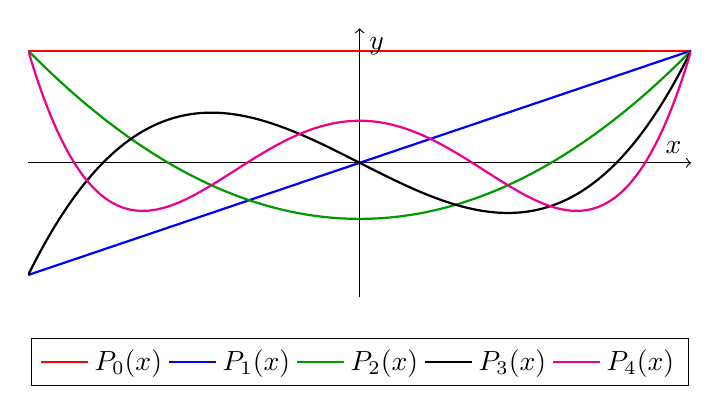
\begin{tikzpicture}
\begin{axis}[
    width=10cm, height=5cm,
    domain=-1:1,
    samples=200,
    axis lines=middle,
    xlabel={$x$},
    ylabel={$y$},
    ymin=-1.2, ymax=1.2,
    legend style={
    at={(0.5,-0.15)}, 
    anchor=north, 
    legend columns=-1
    },
    axis line style={->},
    ticks=none,
]
% Legendre P0
\addplot[red, thick] {1};
\addlegendentry{$P_0(x)$}
% Legendre P1
\addplot[blue, thick] {x};
\addlegendentry{$P_1(x)$}
% Legendre P2
\addplot[green!60!black, thick] {(3*x^2 - 1)/2};
\addlegendentry{$P_2(x)$}
% Legendre P3
\addplot[black, thick] {(5*x^3 - 3*x)/2};
\addlegendentry{$P_3(x)$}
% Legendre P4
\addplot[magenta, thick] {(35*x^4 - 30*x^2 + 3)/8};
\addlegendentry{$P_4(x)$}
\end{axis}
\end{tikzpicture}
\end{center}
\keyidea{We can construct Legendre polynomials of \textit{any} order.}
\end{frame}
%%%%%%%%%%%%%%%%%%%%%%%%%%%%%%%%%%%%%%%%%%%%%%%%%%%%%%%%%%%%%%%%%%%%%%%%
\begin{frame}{Revisit Gauss' Theorem}
Let $a=-1$ and $b=1$.
\begin{block}{Theorem}
Let $q(x)$ be a nontrivial polynomial of degree $n+1$ such that
\begin{equation*}
    \int_{-1}^{1} x^k q(x) dx = 0 \qquad (0\le k \le n) \tag{*}
\end{equation*}
and let $x_0, x_1, \ldots, x_n$ be the zeros of $q(x)$.  Then the quadrature
\begin{equation*}
  \int_{-1}^{1} f(x)dx \approx \sum_{i=0}^n A_i f(x_i), \text{ where } A_i=\int_{-1}^{1} \ell_i(x) dx
\end{equation*}
is exact for all polynomials of degree at most $2n+1$. 
\end{block}

    \begin{itemize}
        \item Let $q$ be the Legendre polynomial $q(x)= \phi_{n+1} (x) \in \mathcal{F}$ 

        \item Then equation $(*)$ will always be satisfied
    \end{itemize}
\end{frame}
%%%%%%%%%%%%%%%%%%%%%%%%%%%%%%%%%%%%%%%%%%%%%%%%%%%%%%%%%%%%%%%%%%%%%%%%
\begin{frame}{Connection between the Theorem and Legendre}
\begin{itemize}
    \item Gauss' Theorem gave us a powerful quadrature 
        $$ \int_{-1}^{1} f(x)\,dx \approx \sum_{i=0}^n A_i f(x_i) $$
        with weights 
        $$A_i = \int_{-1}^{1} \ell_i(x) \,dx$$

    \item \emph{But}, the nodes were never specified because we did not know $q(x)$
\end{itemize}
    
\keyidea{
    We let $q(x)$ be the Legendre polynomial to get the Gaussian quadrature formula of any order.
}

\end{frame}
%%%%%%%%%%%%%%%%%%%%%%%%%%%%%%%%%%%%%%%%%%%%%%%%%%%%%%%%%%%%%%%%%%%%%%%%
\begin{frame}{Properties of Legendre Polynomials}
\vspace{-0.5cm}
\begin{center}
  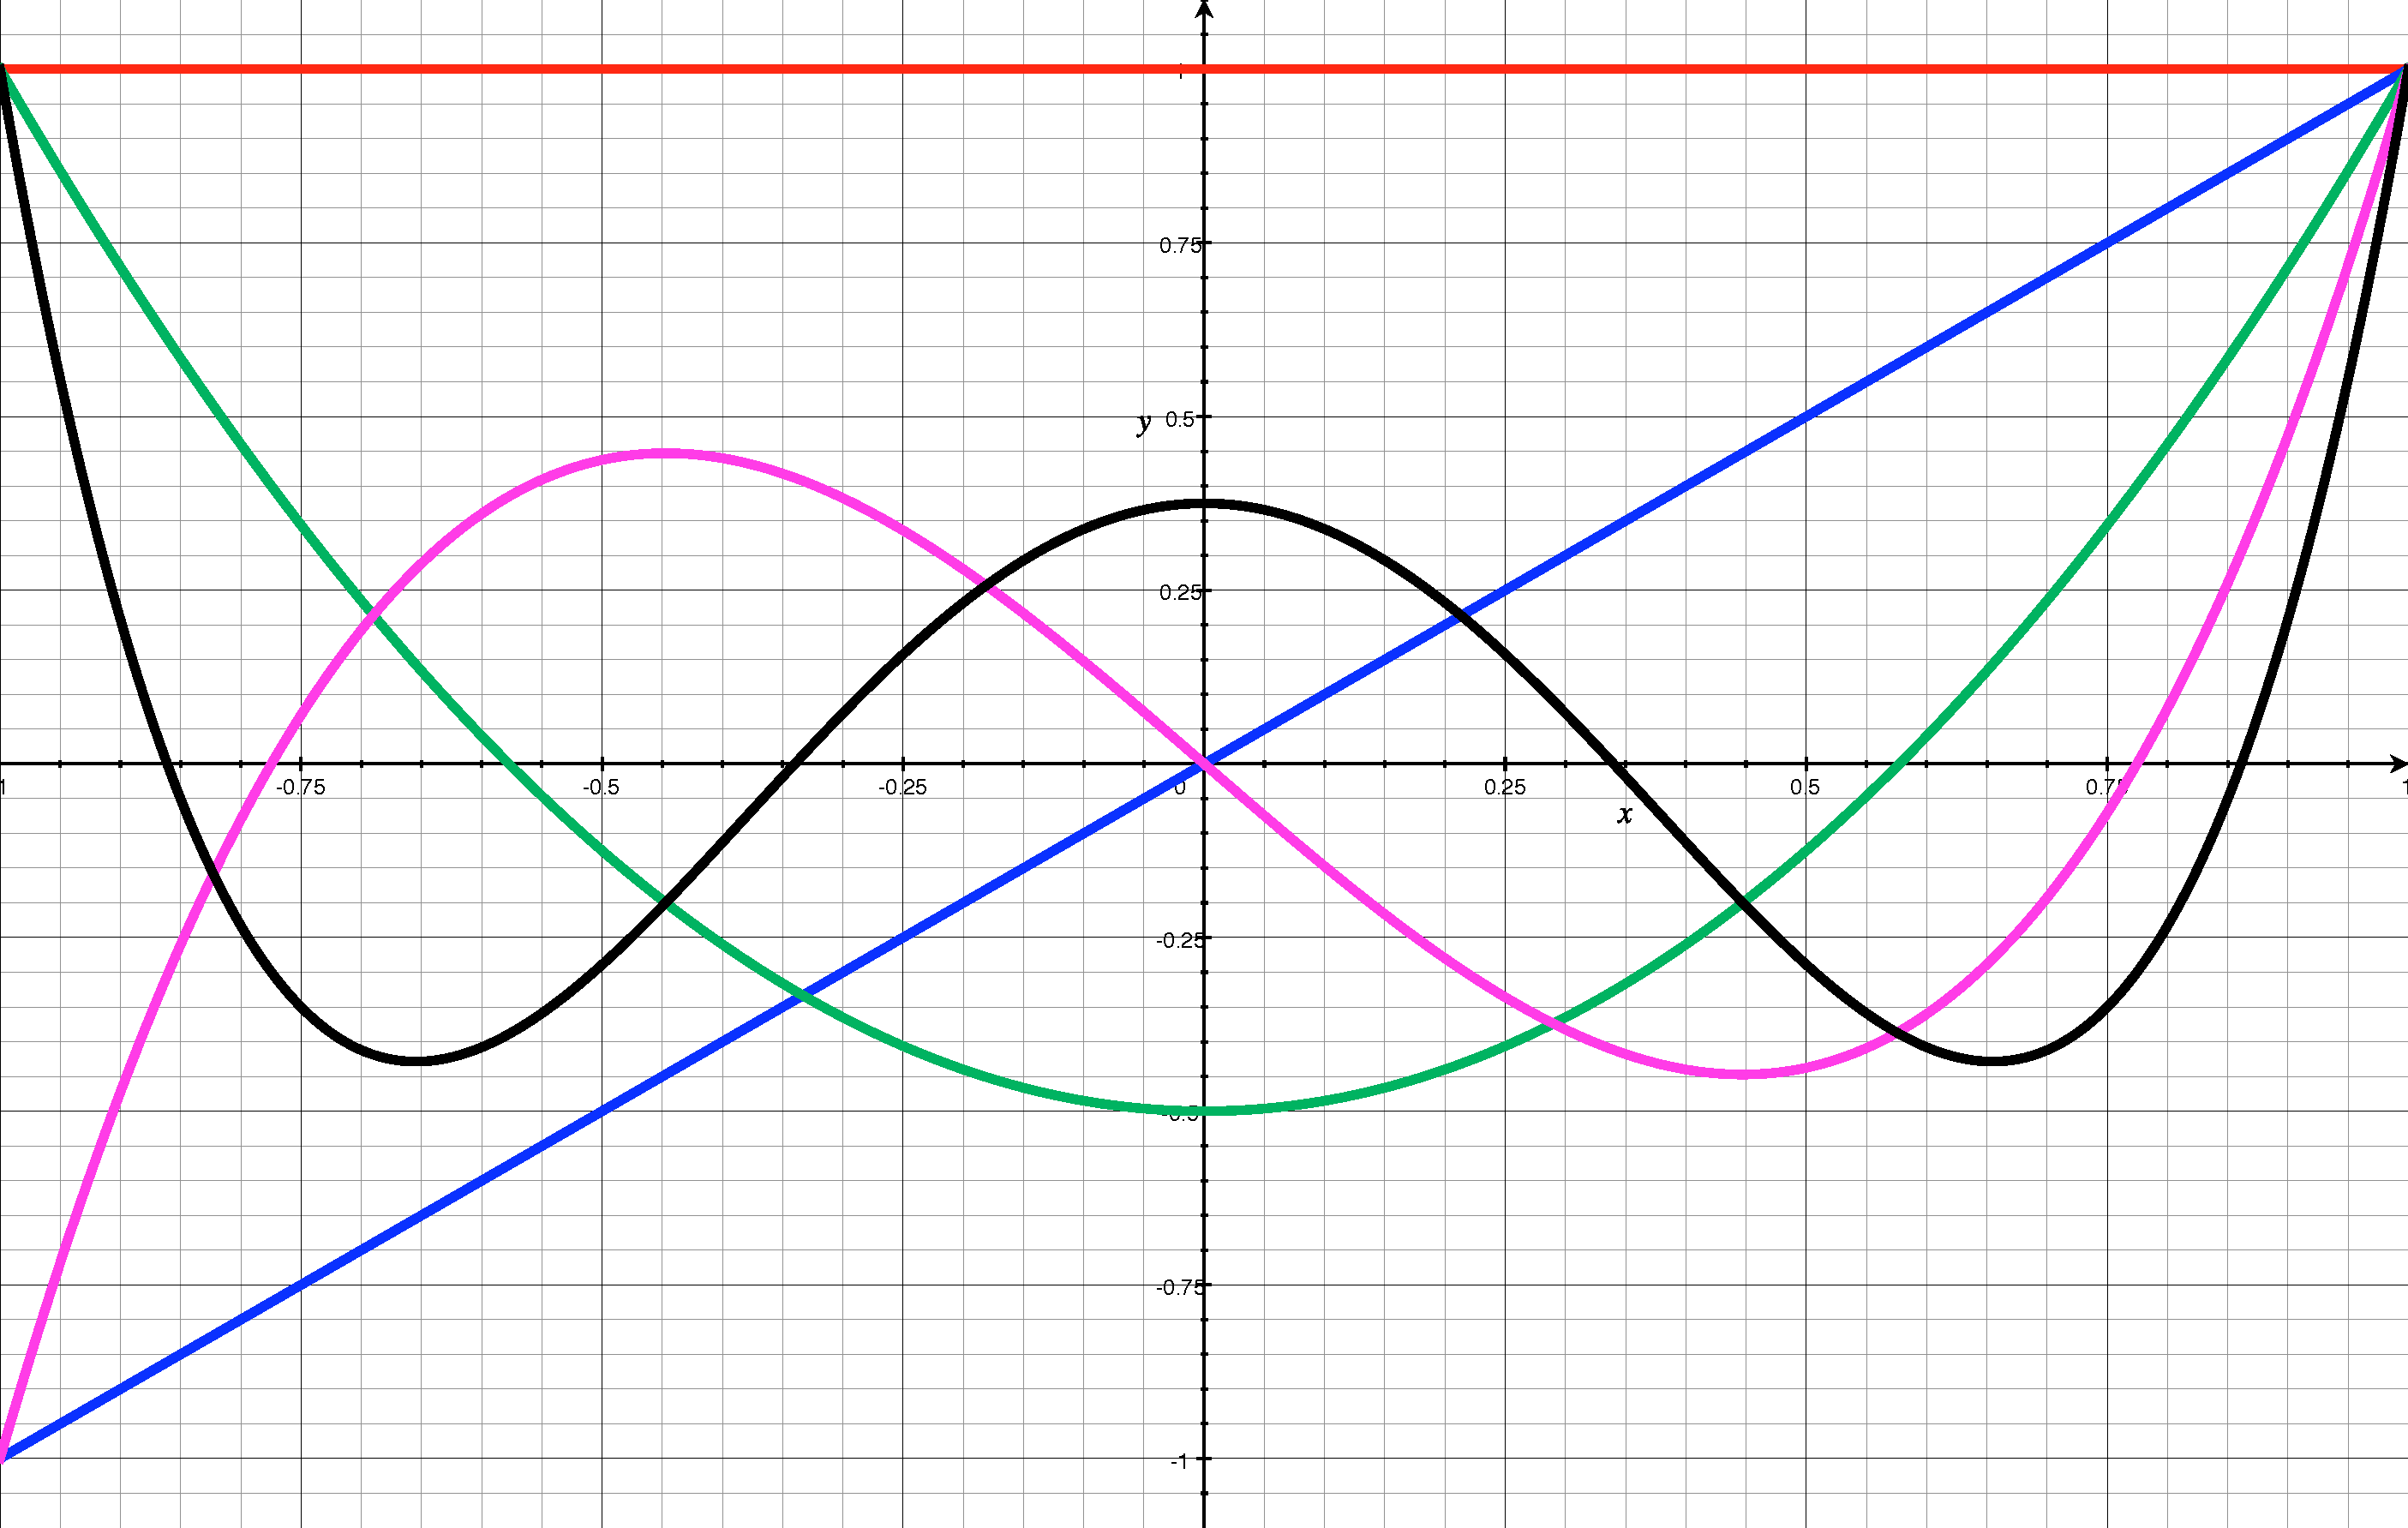
\includegraphics[height=3.5cm]{./figs/legendre.pdf}
\end{center}
  Properties:
  \begin{itemize}
    \item $\phi_n$ is a degree $n$ polynomial
    \item $\phi_i$ is orthogonal to $\phi_j$ if $i\neq j$
    \item Don't suffer from poor conditioning (unlike monomials)
    \item Recursion equation can be used to find $\phi_n(x)$, for $n>1$
    \item The roots of $\phi_n(x)$ are the nodes for Gaussian quadrature
    \item The roots of $\phi_n(x)$ are distributed symmetrically
  \end{itemize}
\end{frame}
%%%%%%%%%%%%%%%%%%%%%%%%%%%%%%%%%%%%%%%%%%%%%%%%%%%%%%%%%%%%%%%%%%%
\begin{frame}{Roots}
\begin{center}
    
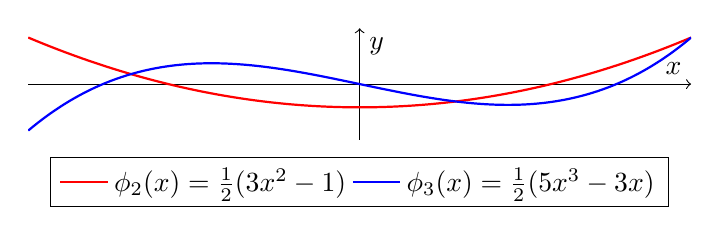
\begin{tikzpicture}
\begin{axis}[
    width=10cm, height=3cm,
    domain=-1:1,
    samples=200,
    axis lines=middle,
    xlabel={$x$},
    ylabel={$y$},
    ymin=-1.2, ymax=1.2,
    legend style={
    at={(0.5,-0.15)}, 
    anchor=north, 
    legend columns=-1
    },
    axis line style={->},
    ticks=none,
]
% Legendre P2
\addplot[red, thick] {(3*x^2 - 1)/2};
\addlegendentry{$\phi_2(x)=\frac12(3x^2-1)$}
% Legendre P3
\addplot[blue, thick] {(5*x^3 - 3*x)/2};
\addlegendentry{$\phi_3(x)=\frac{1}{2}(5x^3-3x)$}
\end{axis}
\end{tikzpicture}
\end{center}
\begin{itemize}
    \item The roots of $\phi_2(x)$ are
    $$
    x_0 = -\frac{1}{\sqrt{3}}, \quad x_1 = \frac{1}{\sqrt{3}}
    $$
    \item The roots of $\phi_3(x)$ are
    $$
    x_0 = -\sqrt{\frac{3}{5}}, \quad x_1 = 0,\quad x_2 = \sqrt{\frac{3}{5}}
    $$
\end{itemize}
\end{frame}
%%%%%%%%%%%%%%%%%%%%%%%%%%%%%%%%%%%%%%%%%%%%%%%%%%%%%%%%%%%%%%%%%%%
\begin{frame}{Weights}
\question{How do you find the Gauss weights?}
\begin{itemize}
    \item We want to know the weights and nodes for the approximation
        $$\int_{-1}^1 f(x)\,dx \approx  w_0f(x_0) + w_1 f(x_1) + w_2 f(x_2)$$
    \item The third Legendre polynomial is 
        $$\phi_3(x) = \frac{5x^3 -3x}{2}$$
        which has roots at $x=0, \pm\ \sqrt{\frac{3}{5}}$ so 
        $$x_0 = -\sqrt{\frac{3}{5}},\quad x_1 = 0,\quad x_2 = \sqrt{\frac{3}{5}}$$
\end{itemize}
\end{frame}
%%%%%%%%%%%%%%%%%%%%%%%%%%%%%%%%%%%%%%%%%%%%%%%%%%%%%%%%%%%%%%%%%%%%%%%%
\begin{frame}{Weights}

\begin{itemize}
    \item The weights $w_i$ can be found by integrating the Lagrange basis functions
        \begin{align*}
            w_0 &= \int_{-1}^1 \ell_0(x)\,dx = \int_{-1}^1 \frac{(x-x_1)(x-x_2)}{(x_0-x_1)(x_0-x_2)}\,dx =\frac{5}{9} \\
            w_1 &= \int_{-1}^1 \ell_1(x)\,dx =\frac{8}{9}\\
            w_2 &= \int_{-1}^1 \ell_2(x)\,dx =\frac{5}{9}
        \end{align*}
    \item Therefore the formula for the Three-Point Gauss Quadrature is 
        $$\int_{-1}^1 f(x)\,dx \approx \frac59\,f\left(-\sqrt{3/5}\right) + \frac89\, f(0) + \frac59 \,f\left(\sqrt{3/5}\right)$$
\end{itemize}
\end{frame}

%%%%%%%%%%%%%%%%%%%%%%%%%%%%%%%%%%%%%%%%%%%%%%%%%%%%%%%%%%%%%%%%%%%%%%%%
\begin{frame}{Nodes and Weights}
\begin{center}
  \pgfimage[width=7.8cm]{./figs/GaussNodes}
\end{center}
\begin{itemize}
    \item The bold ticks show the locations of the nodes
    \item The numbers above them show the weight
    \item Both the node locations and weights are symmetric
\end{itemize}
\end{frame}
%%%%%%%%%%%%%%%%%%%%%%%%%%%%%%%%%%%%%%%%%%%%%%%%%%%%%%%%%%%%%%%%%%%%%%%%
\begin{frame}[containsverbatim,shrink]
\frametitle{Quadrature Nodes}
\begin{itemize}
  \item In practice, programmers use a look-up table for the $x_i$ and $w_i$
  \begin{lstlisting}
  if(n==0)
    x = 0;   w = 2;
  if(n==1)
    x(1) = -1/sqrt(3);     x(2) = -x(1);
    w(1) =  1;             w(2) =  w(1);
  if(n==2)
    x(1) = -sqrt(3/5);    x(2) =  0;      x(3) = -x(1);
    w(1) =  5/9;          w(2) =  8/9;    w(3) =  w(1);
  if(n==3)
    x(1) = -0.861136311594053;     x(4) = -x(1);
    x(2) = -0.339981043584856;     x(3) = -x(2);
    w(1) =  0.347854845137454;     w(4) =  w(1);
    w(2) =  0.652145154862546;     w(3) =  w(2);
  if(n==4)
    x(1) = -0.906179845938664;     x(5) = -x(1);
    x(2) = -0.538469310105683;     x(4) = -x(2);
    x(3) =  0;
    w(1) =  0.236926885056189;     w(5) =  w(1);
    w(2) =  0.478628670499366;     w(4) =  w(2);
    w(3) =  0.568888888888889;
  if(n==5)
    x(1) = -0.932469514203152;     x(6) = -x(1);
    x(2) = -0.661209386466265;     x(5) = -x(2);
    x(3) = -0.238619186083197;     x(4) = -x(3);
    w(1) =  0.171324492379170;     w(6) =  w(1);
    w(2) =  0.360761573048139;     w(5) =  w(2);
    w(3) =  0.467913934572691;     w(4) =  w(3);
  \end{lstlisting}
\end{itemize}
\end{frame}



%%%%%%%%%%%%%%%%%%%%%%%%%%%%%%%%%%%%%%%%%%%%%%%%%%%%%%%%%%%%%%%%%%%%%%%%


%%%%%%%%%%%%%%%%%%%%%%%%%%%%%%%%%%%%%%%%%%%%%%%%%%%%%%%%%%%%%%%%%%%%%%%%
\begin{frame}{Example}
\begin{example}
What is the minimum number of Gauss nodes needed to guarantee exact
integration of every polynomial of degree at most $12$?
\end{example}
\begin{itemize}
    \item An $m$-point Gauss rule has degree of precision $2m-1$.
    \item We need
    \[
        2m-1\ge 12 \quad\Longrightarrow\quad m\ge \frac{13}{2}.
    \]
    \item The smallest integer is $m=7$: use \textbf{7-point Gauss}.
\end{itemize}
\end{frame}

%%%%%%%%%%%%%%%%%%%%%%%%%%%%%%%%%%%%%%%%%%%%%%%%%%%%%%%%%%%%%%%%%%%%%%%%
\begin{frame}[shrink]{Let's run some code}

\begin{block}{int\_gauss\_test.m}
  This script uses int\_gauss.m to integrate $\int_{0}^{5} x e^{-x}\,dx$ with
  \begin{enumerate}
    \item 1 panel, increasing number of nodes
    \item 3 nodes per panel, increasing number of panels 
  \end{enumerate}
\end{block}

\begin{figure}
    \centering
    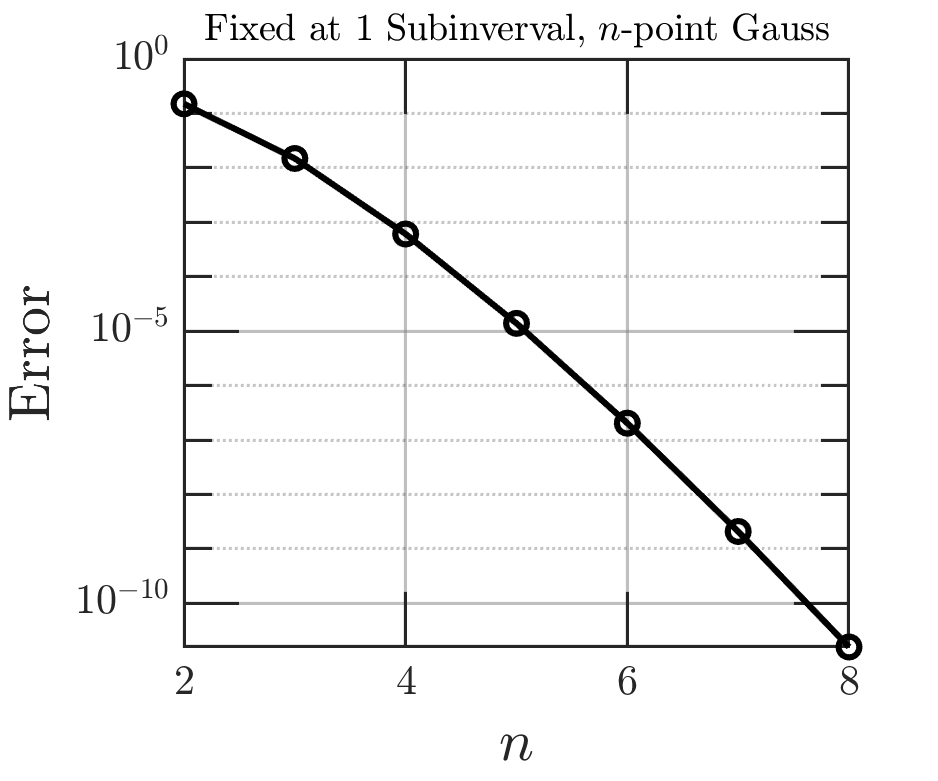
\includegraphics[width=0.47\linewidth]{figs/gauss_test_a.png}
    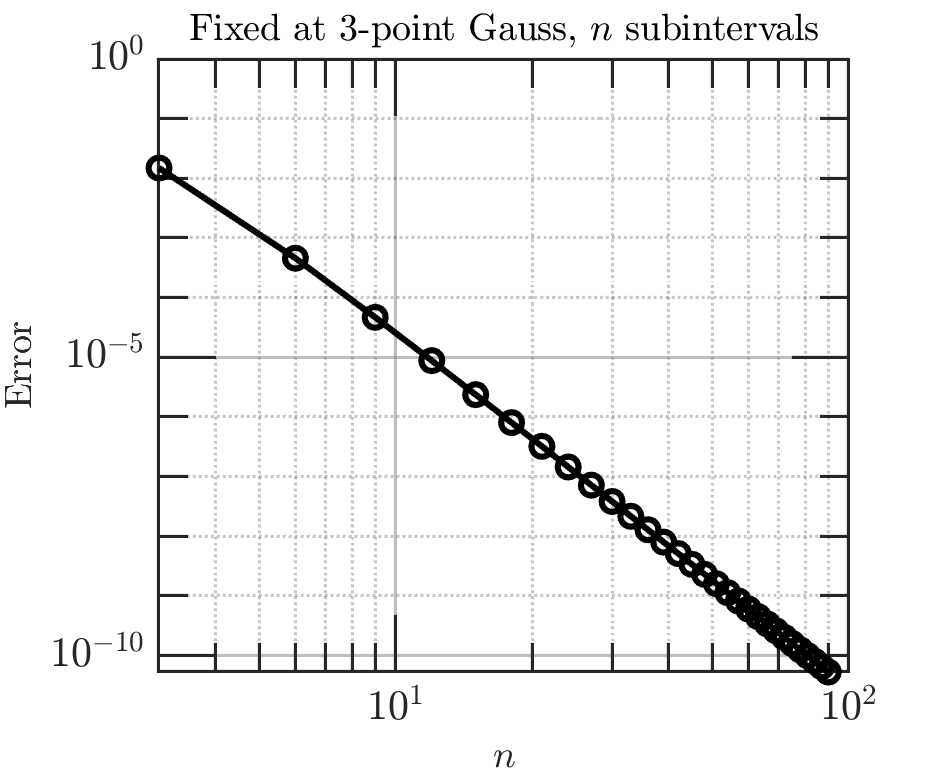
\includegraphics[width=0.47\linewidth]{figs/gauss_test_b.png}
\end{figure}
\end{frame}

%%%%%%%%%%%%%%%%%%%%%%%%%%%%%%%%%%%%%%%%%%%%%%%%%%%%%%%%%%%%%%%%%%%%%%%%
\begin{frame}[shrink]{Let's run some code}

\begin{block}{int\_compare\_gauss\_trapezoid\_simpson.m}
  Compare the numerical experiment for integrating $\int_{0}^{5} x e^{-x}\,dx$ with
  \begin{enumerate}
    \item Trapezoid
    \item Simpson
    \item Gauss
  \end{enumerate}
  Result: Gauss quadrature is much more accurate for the same number of function evals.
\end{block}
\begin{figure}
    \centering
    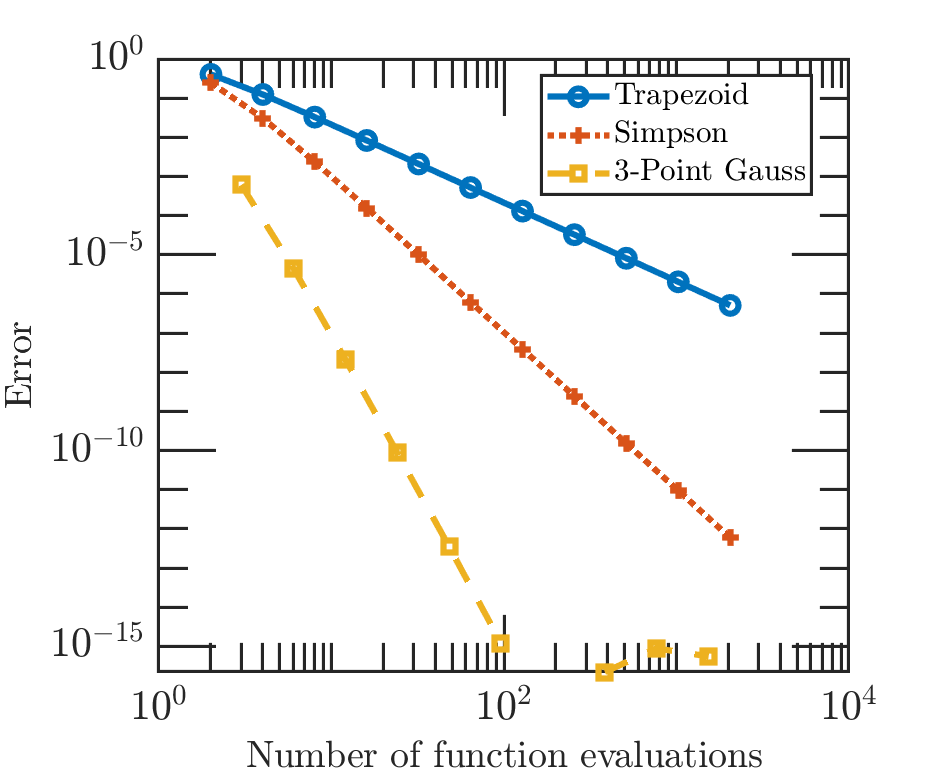
\includegraphics[width=0.45\linewidth]{figs/gauss_test_compare.png}
\end{figure}
\end{frame}

%%%%%%%%%%%%%%%%%%%%%%%%%%%%%%%%%%%%%%%%%%%%%%%%%%%%%%%%%%%%%%%%%%%%%%%%%
\sectionframe{Higher Dimensions}
%%%%%%%%%%%%%%%%%%%%%%%%%%%%%%%%%%%%%%%%%%%%%%%%%%%%%%%%%%%%%%%%%%%%%%%%%
\begin{frame}{Something interesting...}

    \begin{center}
    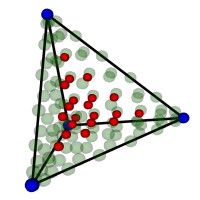
\includegraphics[width=3cm]{./figs/tet}
    \end{center}

\begin{itemize} 
  \item Gaussian quadrature also works for $\iint f(x,y) \,dA$ 
  \item Also works for $\iiint f(x,y,z) \, dV$
  \item Gauss nodes in other shapes are not easy
\end{itemize}
\end{frame}
%%%%%%%%%%%%%%%%%%%%%%%%%%%%%%%%%%%%%%%%%%%%%%%%%%%%%%%%%%%%%%%%%%%%%%%%
%%%%%%%%%%%%%%%%%%%%%%%%%%%%%%%%%%%%%%%%%%%%%%%%%%%%%%%%%%%%%%%%%%%%%%%%
\begin{frame}
\frametitle{Quadrature}
Consider quadrature over ``interesting'' 3D domain
\begin{center}
  \pgfimage[width=0.8\textwidth]{./figs/brick1}
\end{center}
\end{frame}
%%%%%%%%%%%%%%%%%%%%%%%%%%%%%%%%%%%%%%%%%%%%%%%%%%%%%%%%%%%%%%%%%%%%%%%%
%%%%%%%%%%%%%%%%%%%%%%%%%%%%%%%%%%%%%%%%%%%%%%%%%%%%%%%%%%%%%%%%%%%%%%%%
\begin{frame}
\frametitle{Quadrature}
Consider quadrature over ``interesting'' 3D domain

- Break into "subintervals" of 40K tetrahedrons, and integrate each tet
\begin{center}
  \pgfimage[width=0.8\textwidth]{./figs/brick2}
\end{center}
\end{frame}
%%%%%%%%%%%%%%%%%%%%%%%%%%%%%%%%%%%%%%%%%%%%%%%%%%%%%%%%%%%%%%%%%%%%%%%%
%%%%%%%%%%%%%%%%%%%%%%%%%%%%%%%%%%%%%%%%%%%%%%%%%%%%%%%%%%%%%%%%%%%%%%%%
\begin{frame}
\frametitle{Quadrature}
\begin{columns}
\begin{column}{0.45\textwidth}
\begin{center}
  \pgfimage[width=5cm]{./figs/brick2}
\end{center}
\end{column}
\begin{column}{0.45\textwidth}
\begin{center}
  \pgfimage[width=3cm]{./figs/tetrahedron}
\end{center}
\end{column}
\end{columns}
\begin{itemize}
  \item 40K tetrahedrons.
  \item Need to integrate a function $f(x)$ over each tet $\Omega_i$: $\int_{\Omega_i} f(x)\,dx$
  \item Needs quadrature
  \item Map the integration to a reference tetrahedron
  \item Perform Gauss Quadrature using $(n+1)(n+2)(n+3)/6$ quadrature
points (where $n$ is the 1-D number of points).
  %\item $f(x)$ is often a product of degree $m$ Lagrange interpolating polynomials
  %\item ...needs large $n$
  \item Results in \# of tetrahedrons $\times$ $n^3/6$ function evaluations
\end{itemize}
\end{frame}
%%%%%%%%%%%%%%%%%%%%%%%%%%%%%%%%%%%%%%%%%%%%%%%%%%%%%%%%%%%%%%%%%%%%%%%%
\begin{frame}{Meet Legendre}
\begin{center}
    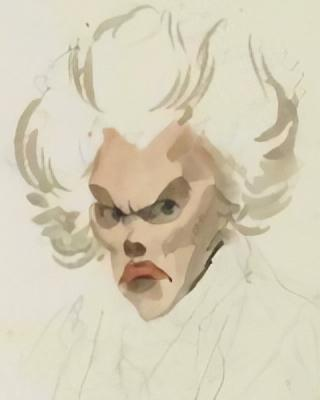
\includegraphics[scale=0.4]{figs/Legendre.jpg}\\
    This is the only picture of Adrien-Marie Legendre (1752-1833)
\end{center}
    
\end{frame}
%%%%%%%%%%%%%%%%%%%%%%%%%%%%%%%%%%%%%%%%%%%
\end{document}

